\documentclass[tikz,border=6pt]{standalone}
\usepackage{amsmath}
\usetikzlibrary{arrows.meta,calc,patterns,positioning}
\begin{document}

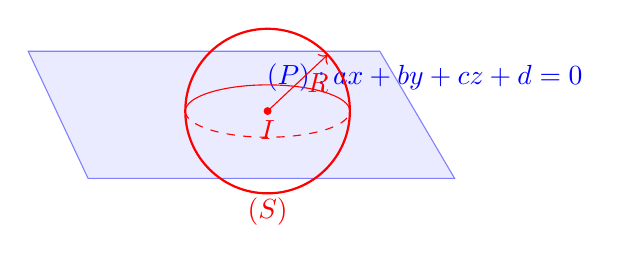
\begin{tikzpicture}[scale=0.95]
  \draw[fill=blue!8,draw=blue!50] (-2.4,-0.7) -- (2.5,-0.7) -- (1.5,1.0) -- (-3.2,1.0) -- cycle;
  \node[blue] at (2.1,0.65) {$(P): ax+by+cz+d=0$};
  \draw[thick,red] (0,0.2) circle (1.1);
  \draw[red,dashed] (-1.1,0.2) arc (180:360:1.1 and 0.35);
  \draw[red] (1.1,0.2) arc (0:180:1.1 and 0.35);
  \fill[red] (0,0.2) circle (1.5pt) node[below] {$I$};
  \draw[->,red] (0,0.2) -- (0.8,0.95) node[midway,right] {$R$};
  \node[red] at (0,-1.15) {$(S)$};
\end{tikzpicture}

\end{document}
